\chapter{Query Builder}
\label{chapter:QueryBuilder}

This project has another goal: to enhance the conversational search assistant to collect additional information in order to provide a query as an outcome. The query is referred to as cohort definition in the ATLAS community, as detailed in section \ref{atlas}.

The following section discusses the implementation of the query builder, as well as the decisions and strategies involved.


\section{Implementation Strategy}

% explicar a estratégia de implementação do query builder
%   criação de 2 ficheiros: o cohort template e outro com as respetivas perguntas para cada field
%   pointer para o campo a ser analisado
%   divisão do query builder em 2 partes: concept set and cohort definition

So, to create a system that builds a query through a conversation with the user, the first step is to get a cohort definition generated in the ATLAS platform after implementing an experimental case. Understanding how the cohort is built is crucial at this stage. The section \ref{atlas} details defining a cohort.


\subsection{Interaction between Components}

It is important to understand how this system interacts with the user and other external tools. Diagram \ref{fig_interaction} describes all the interactions between components. The interaction diagram all the interactions between components. The system components are the {\ir} API and the Chatbot Interface, which contains the User interface and the {\llm}. The {\ehden} Portal and ATLAS are external tools.

\begin{figure}[H]
  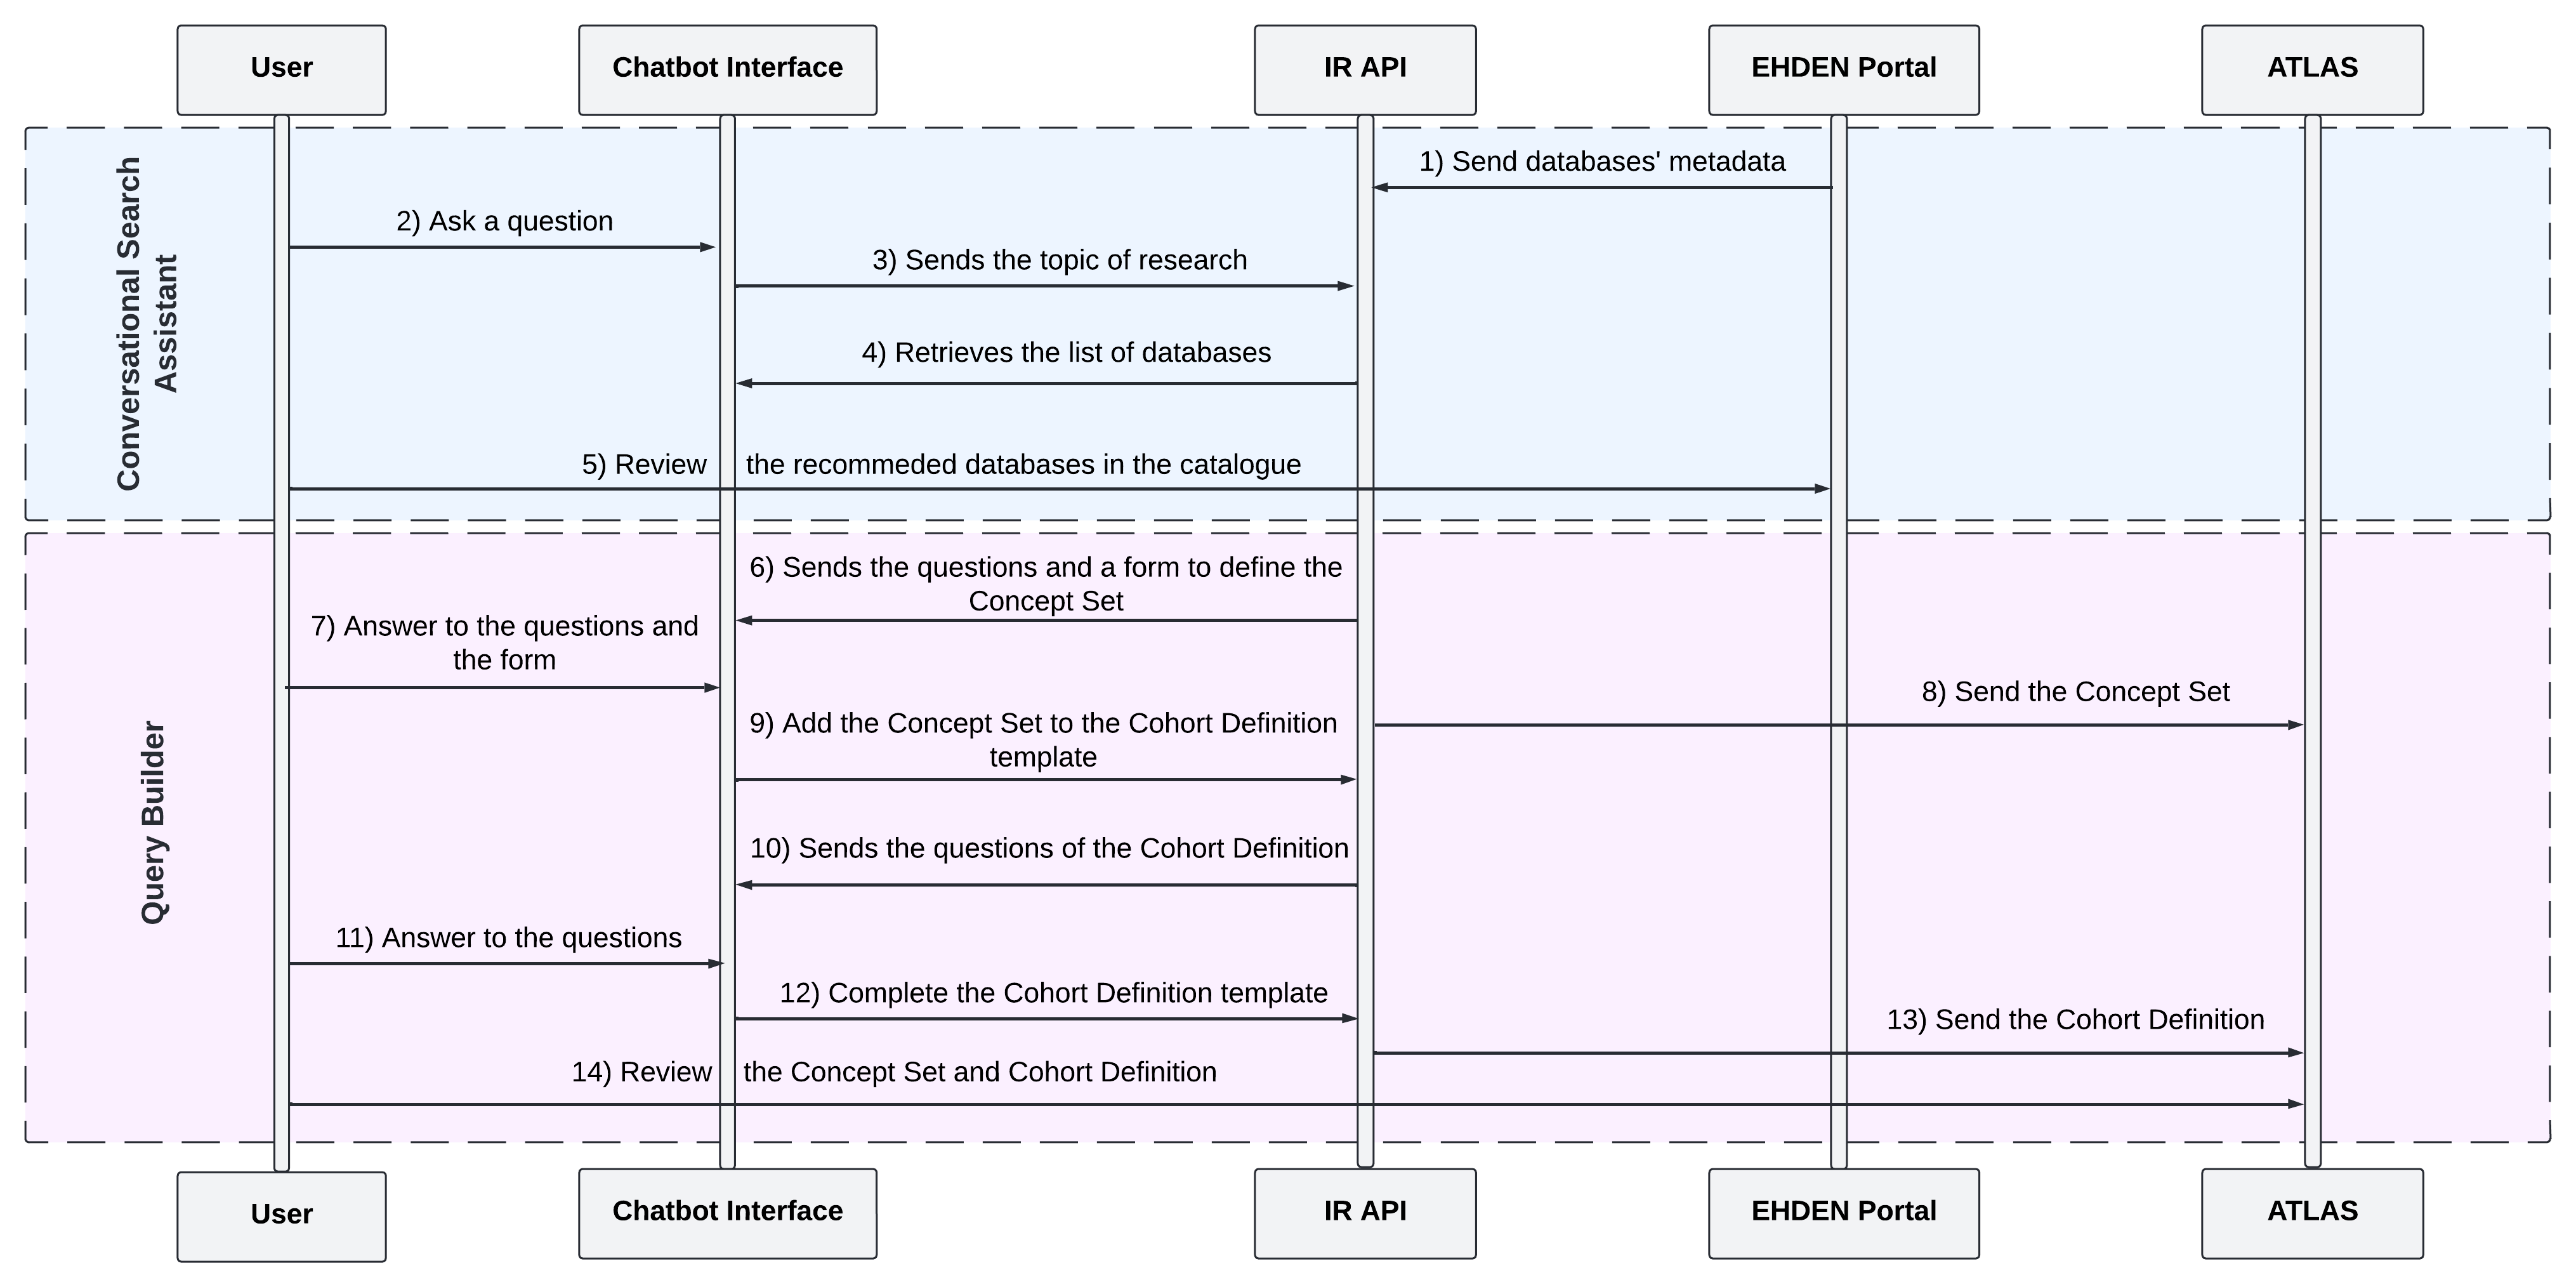
\includegraphics[width=\textwidth]{figs/chapter4/interaction_diagram.png}
  \centering
  \caption{Interaction diagram between the user, the system components and external tools.}
  \label{fig_interaction}
\end{figure}

This diagram presents all the interactions of the conversational query builder, not only presenting the interactions detailed in the previous chapter \ref{chapter:ConversationalSearchAssistant} — steps 1) to 5) —, but also the interactions that will be performed during the detail of this chapter — steps 6) to 9).

Reminding the interactions explained in chapter \ref{chapter:ConversationalSearchAssistant}, the {\ir} component receives the databases' metadata from the {\ehden} Portal — step 1) —, creating and indexing the documents. The user asks a question to the Chatbot Interface — step 2). Here, the {\llm} applies his task of identifying the research topic and sends it to the {\ir} API — step 3). The {\ir} API retrieves the most suitable databases for the research concept and sends the list of databases to the Chatbot Interface — step 4). The user can review the recommended databases in the catalogue in the {\ehden} Portal — step 5). 

Now, the query builder phase starts. The {\ir} API, when sending the databases to the chatbot interface, also sends a question to complete a field in the cohort definition — step 6). The user answer to the question — step 7) — and the {\llm}, in the Chatbot Interface, analyses if the user message is an answer to the question. If so, the answer will be saved in the cohort template — step 8). Steps 6), 7), and 8) are repeated until the cohort template is complete. Finally, the {\ir} API sends the cohort definition to ATLAS — step 9).



\subsection{Template and Questions}

The generated cohort definition, in the ATLAS platform, is in JSON format, which produces two crucial JSON files. One is the template for users to fill out during the conversation {\small\normalfont(\texttt{cohort\_template.json})}. This template is a copy of the cohort definition file without the cohort data {\small\normalfont(\texttt{cohort\_questions.json})}. The other file is the questions associated with each key field of the template. Each question should be simple and efficient so the medical researcher can respond to it, and its response is the value of that key. Also, each question in the template is manually inserted in the JSON file.  

% TODO: referenciar os templates


\begin{listing}[H]
  \begin{minted}[breaklines]{json}
      
  {
    "ConceptSets": [
      {
        "expression": {
            "items": "Do you have any other concepts to add to the concept set? (The question should be a yes with the new concepts or no response.)"
        }
      }
    ],
    "PrimaryCriteria": {
      "CriteriaList": [
        {
          "DrugExposure": {
            "CodesetId": 0,
            "First": true
          }
        }
      ],
      "ObservationWindow": {
        "PriorDays": "In terms of the observation window, what is the number of previous days? you can choose from 0, 1, 7, 14, 21, 30, 60, 90, 120, 180, 365, 548, 730 or 1095.",
        "PostDays": "In terms of the observation window, what is the number of days after? you can choose from 0, 1, 7, 14, 21, 30, 60, 90, 120, 180, 365, 548, 730 or 1095."
      },
      "PrimaryCriteriaLimit": {
        "Type": "First"
      }
    },
    "QualifiedLimit": {
      "Type": "First"
    },
    "ExpressionLimit": {
      "Type": "First"
    },

    (...)
  \end{minted}
  \caption{The cohort questions file {\small\normalfont(\texttt{cohort\_questions.json})}.}
  \label{questions}
  \end{listing}

\begin{listing}[H]
  \begin{minted}[breaklines]{json}
      
  {
    "ConceptSets": [
      {
        "expression": {
            "items": "Do you have any other concepts to add to the concept set? (The question should be a yes with the new concepts or no response.)"
        }
      }
    ],
    "PrimaryCriteria": {
      "CriteriaList": [
        {
          "DrugExposure": {
            "CodesetId": 0,
            "First": true
          }
        }
      ],
      "ObservationWindow": {
        "PriorDays": "In terms of the observation window, what is the number of previous days? you can choose from 0, 1, 7, 14, 21, 30, 60, 90, 120, 180, 365, 548, 730 or 1095.",
        "PostDays": "In terms of the observation window, what is the number of days after? you can choose from 0, 1, 7, 14, 21, 30, 60, 90, 120, 180, 365, 548, 730 or 1095."
      },
      "PrimaryCriteriaLimit": {
        "Type": "First"
      }
    },
    "QualifiedLimit": {
      "Type": "First"
    },
    "ExpressionLimit": {
      "Type": "First"
    },
    
    (...)
  \end{minted}
\caption{The cohort template file {\small\normalfont(\texttt{cohort\_template.json})}.}
\label{template}
\end{listing}  


\subsection{Template Pointer}

In a nutshell, the cohort questions file have the questions to complete the cohort template file. However, when exchanging messages with the user, tracking which questions must be asked and which question the user responded to is essential and also a problem.

The solution to this issue is creating a pointer to a template key. The pointer retrieves a template key that should be completed with the user information. The pointer points to the same key until the user responds to the question associated with the pointer. Otherwise, it moves to the following template key.

So, during the conversation, the pointer helps:

\begin{itemize}
  \item To determine the appropriate question to ask the user.
  \item To identify which key of the cohort template to use to save the user's answer.
  \item To move on to the next question of the cohort template.
\end{itemize}

This solution keeps track of the user's responses and dynamically updates the template with the relevant information throughout the conversation.


\section{Concepts Set}

% https://ohdsi.github.io/TheBookOfOhdsi/Cohorts.html#conceptSets

In template \ref{template}, a cohort is defined by multiple JSON fields. One of these fields is the concepts set (the template key is '\textit{ConceptsSet}'), which is a list of concepts required to meet the study requirements of the researcher. The definition of the concept set also needs to be defined in the conversation and so, the strategy was first define the concept set in the conversation and then, the remaining fields of the cohort template.

Before defining a cohort, the concept set needs to be determined. It is a set of standardized medical terms that define clinical elements such as diseases, drugs, and procedures.

This section details the creation of the concept set needed for the cohort definition later.


\subsection{Expression}
A concept set expression is comprised of a list of concepts with the following attributes:

\begin{itemize}
  \item \textbf{concept}: Definition of a concept, using data contained in the concepts file  {\small\normalfont(\texttt{concepts.csv})} (section \ref{data}).
  \item \textbf{isExcluded}: Exclude the concept from the concept set.
  \item \textbf{includeDescendants}: Add all of descendants of a concept, with it also included.
  \item \textbf{includeMapped}: Allow the search for non-standard concepts.
\end{itemize}


The JSON example \ref{conceptset} below represents a concept definition within a concept set expression. This example is not real information; it is just to define a concept set visually.

\begin{listing}[H]
  \begin{minted}[breaklines]{json}
      
    {
      "id": 0,
      "name": "costum_concept_set",
      "expression": {
          "items": [
              {
                  "concept": {
                      "CONCEPT_ID": 231256,
                      "CONCEPT_NAME": "Covid-19",
                      "DOMAIN_ID": "Condition",
                      "VOCABULARY_ID": "ASG67HR",
                      "CONCEPT_CLASS_ID": "ASG67 code",
                      "CONCEPT_CODE": "953635",
                      "VALID_START_DATE": "2000-01-01",
                      "VALID_END_DATE": "2099-12-31"
                  },
                  "isExcluded": false,
                  "includeDescendants": true,
                  "includeMapped": false
              },
              
              (...)
          ]
      }
    }

  \end{minted}
\caption{A Concept Set expression example.}
\label{conceptset}
\end{listing}  



\subsection{Implementation}


% 0) o utilizador insere uma query, o chatbot pergunta se ele tem mais conceitos, se sim, que os indique, até ao utilizador dizer que não tem mais conceitos para adicionar
% 1) utilizar IR para encontrar os conceitos associados à query que o user inseriu
% 2) ir buscar as informações adicionais aos ficheiro de conceitos
% 3) enviar a lista de conceitos ao utilizador e apresentar como forms 
% 4) utilizador escolhe os conceitos que quer inserir e escolhe os atributos
% 5) submete o forms, e a concept set é criado


The goal is to create a JSON object identical to the one in the example \ref{conceptset} with the concepts selected by the medical researcher.

When a user enters a query, the conversational search assistant retrieves the best databases related to the health topic of that query. It should also inquire whether the user has additional concepts for their study requirements. In an implementation vision, the first key to complete in the cohort template is '\textit{ConceptsSet}', so the question regarding that key is rewritten by the {\llm} and then asked to the user.

The user should respond to whether there are additional concepts to add. If there are, he should indicate them. If not, he should provide a negative answer. The chatbot will continue to ask if there are more concepts until the user confirms that there are no more to add.

Now, in the {\ir} component, the {\bm} technique searches in the collection for the concepts the user indicates in his responses. After identifying each concept in the collection using the {\ir} technique search, additional information from the concept file is added. This includes the concept ID, concept code, and other attributes that define the concept as represented in example \ref{conceptset}.

The list of concepts identified is sent to the chatbot interface. The chatbot interface shows the concepts in a form. For example, the Figure \ref{fig_forms} shows a form to create the concept set. The user selected which concepts he wants to include and the others attributes.

% TODO:  meter blur nos conceitos e ids
\begin{figure}[H]
  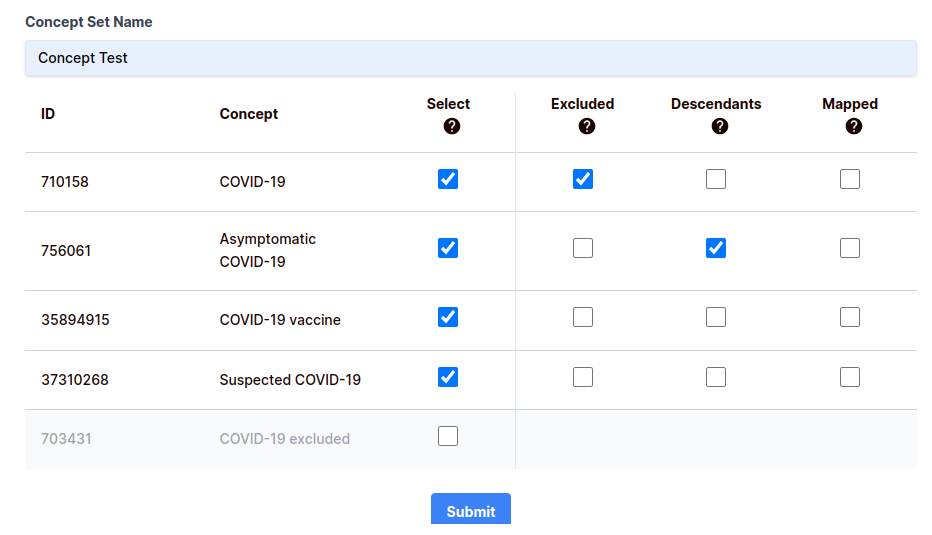
\includegraphics[width=1\textwidth]{figs/chapter4/form.png}
  \centering
  \caption{The form to create the Concept Set.}
  \label{fig_forms}
\end{figure}

Finally, the user submits the forms, creating the concept set. The chatbot sends a message informing the user that he can download the cohort, which is now only the concept set. The pointer of the cohort template moves to the next key.



\section{Cohort Definition}

% depois do concept set estar definido, o template pointer passa para a proxima key com pergunta
% o LLM gera a pergunta e a interface apresenta-a ao utilizador
% o utilizador responde 
% o LLM verifica se a mensagem do utilizador é em resposta à pergunta
%   - se sim, atualiza o template com a resposta, e o template pointer avança
%   - se não, volta a questionar a mesma questão ao utilzador
% este ciclo repete-se até o cohort estar completo


% TODO: intro, e fazer refenciar o template

Once the concept set is defined, the list of concepts and their attributes are saved on the template, where the template key points to. Then, the template pointer moves to the next template key. The {\llm} generates a specific question related to the question that the current key points to. This generated question is then presented to the user through the interface.

The user provides a response to the question presented. The user message could be a possible response to the question or, for example, can be a random message. So, the {\llm} checks if the user's message is indeed an answer to the question. This task is mentioned in the section \ref{sec:llm}. If the response is valid,the {\llm} extracts the value and the template is updated with that value. The template pointer advances to the next key, where the next question will be generated by the {\llm}. Otherwise, if the response is invalid or unrelated, the pointer remains on the same key because the question is not answered yet.

This cycle of getting the question of the pointer, generating the question, presenting it, receiving a response, and verifying the response repeats until the entire cohort is complete, and all keys in the template are filled with the appropriate user responses.

% TODO: end



\section{ATLAS ...}


% tbd
nome da secção

o que escrever aqui

onde meter esta figura

\begin{figure}[H]
  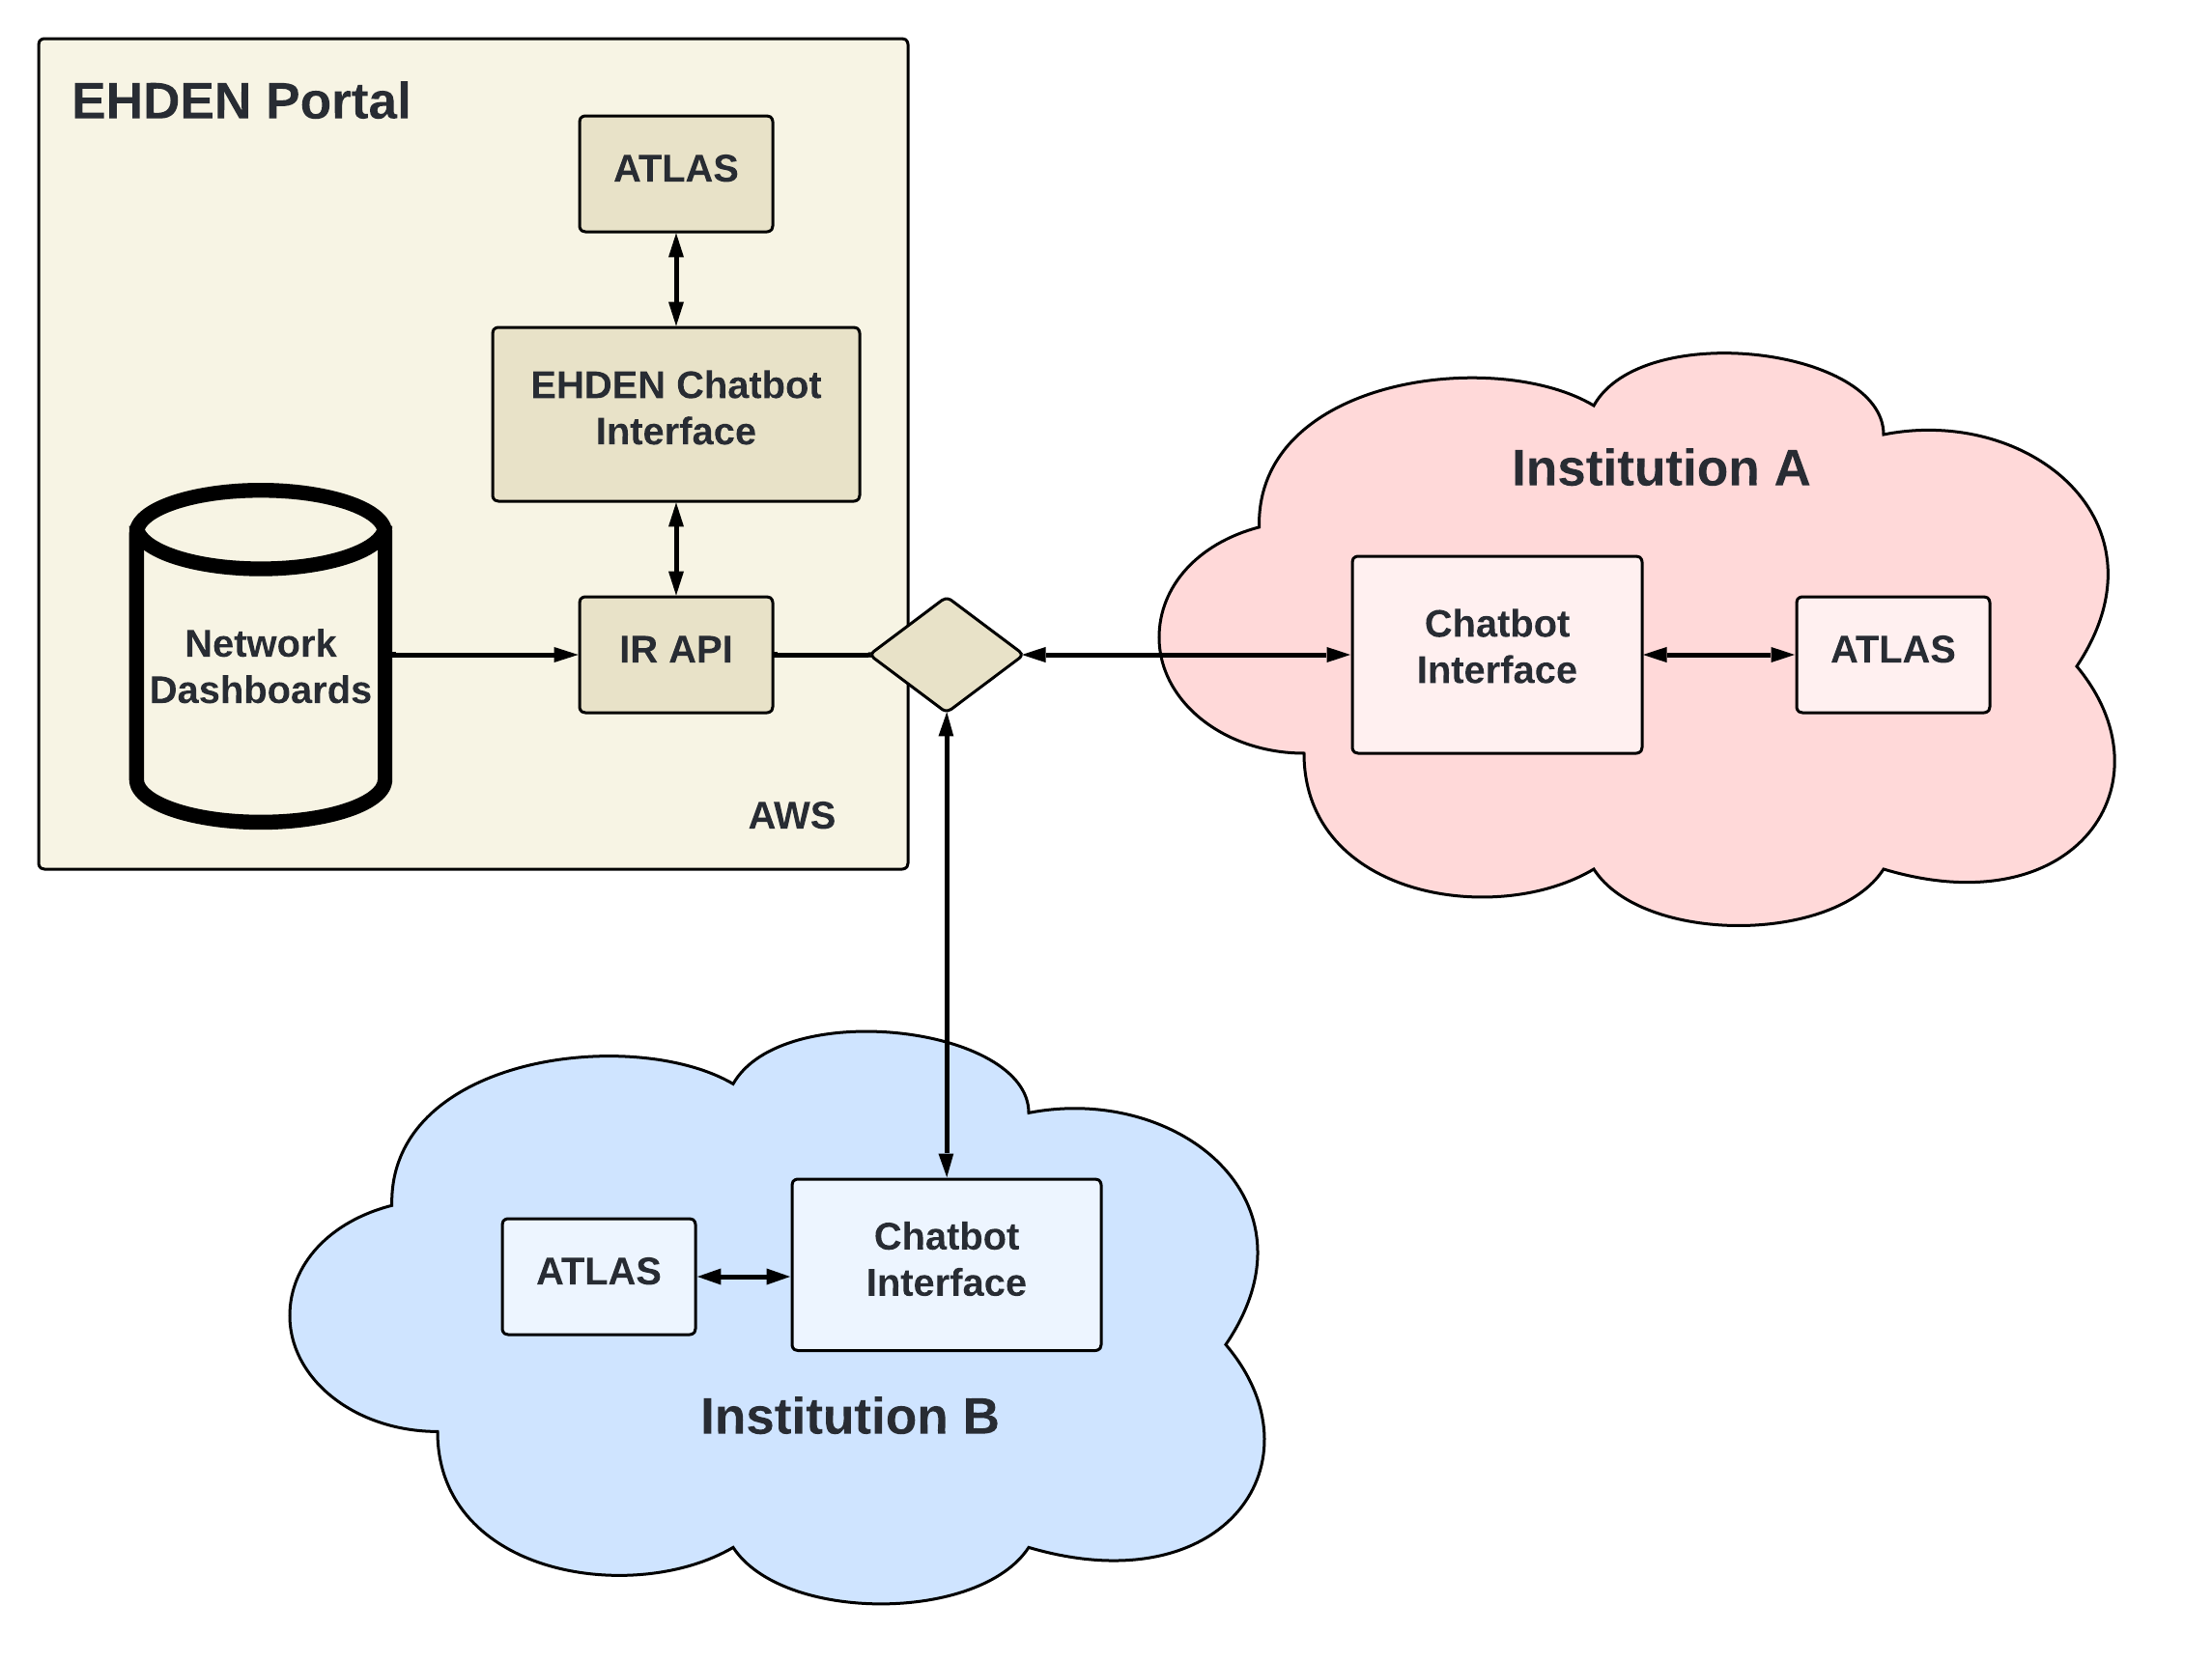
\includegraphics[width=0.5\textwidth]{figs/chapter4/network_diagram.png}
  \centering
  \caption{Network diagram.}
  \label{fig_network}
\end{figure}


---

o que fazer com os json dos templates

quero refenciar o artigo cbms e o MIE


----

falta falar que há um histórico para guardar as conversas de investigadores médico --> onde meto isto?

é preciso meter uma documentação da API?